\textbf{COLUNI 2021 -- Questão 35}\par\medskip No início do século XX, a China era um país monarquista e pouco industrializado. Naquele momento, o descontentamento popular com o governo era crescente, em razão da conivência da monarquia com a exploração do país pelas potências capitalistas ocidentais e pelo crescente imperialismo japonês. Na Segunda Grande Guerra, a China foi massacrada pelo Japão, que chegou a ocupar a então capital chinesa, no que ficou conhecido como Massacre de Nanquim (1937-1938). O gráfico abaixo demonstra como a economia chinesa havia sido uma grande potência no cenário global e sua vertiginosa queda entre meados do século XIX e meados do século XX, período chamado, na China, de “século da humilhação”.

% COLUNI-AUTO-FIGURES-BEGIN
\begin{figure}[htbp]
\centering
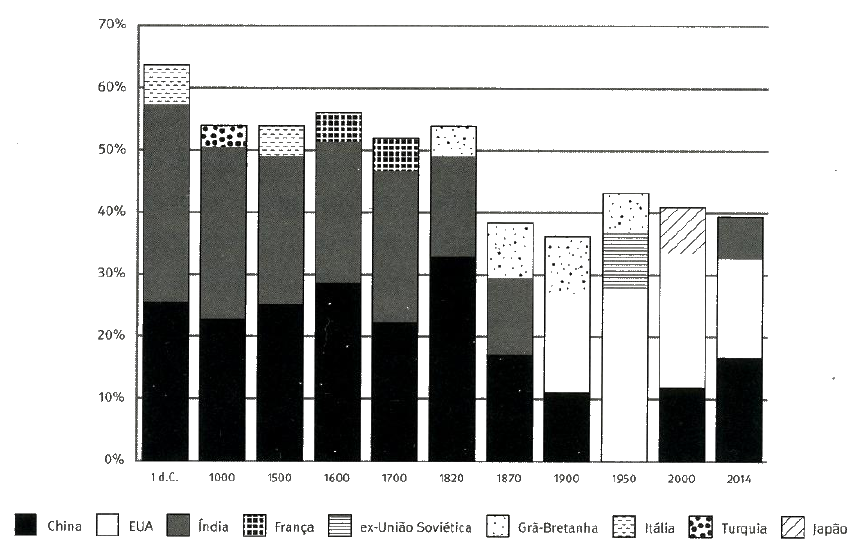
\includegraphics[width=0.95\linewidth]{static/simulados/coluni/figuras/2021/questao-35/figura-1.png}
\end{figure}
% COLUNI-AUTO-FIGURES-END

“As três maiores economias do mundo, PIB com base na paridade do poder de compra (PPC) como porcentagem do total mundial; produção histórica no interior das fronteiras de países modernos. Fontes: Angus Maddison, Banco Mundial”. STUENKEL, Oliver. \textbf{O Mundo Pós-Colonial}: potências emergentes e a nova ordem global. Rio de Janeiro: Zahar, 2018, p.12.

\par

Em 1911, os nacionalistas chineses derrubaram a monarquia e instauraram uma república. Em 1912, os nacionalistas criaram o Partido Nacionalista do Povo, chamado Kuomintang. Em 1921, foi criado o Partido Comunista Chinês, sob a liderança de Mao Tsé-Tung. Inicialmente, esses dois partidos se uniram para lutar contra o retorno da monarquia na China. Contudo, a partir de 1925, distanciaram-se e passaram a defender projetos diferentes para o país. Nesse contexto, os nacionalistas do Kuomintang aliaram-se aos conservadores chineses e os comunistas aproximaram-se da União das Repúblicas Socialistas Soviéticas, que buscava expandir sua área de influência sobre a China. Entre 1946 e 1949, nacionalistas e comunistas travaram uma guerra civil, com posterior vitória dos comunistas sob a liderança de Mao Tsé-Tung, que tinha a simpatia de muitos chineses em função das pautas que orientavam sua atuação política e buscavam restabelecer a economia e sociedade chinesas. Após a derrota, membros do grupo nacionalista, sob a liderança de Chiang Kai-Chek, instalaram o governo da China Nacionalista em Taiwan.

\par

Sobre o projeto político defendido por Mao Tsé-Tung, após 1949, é CORRETO afirmar que era favorável à:

\begin{enumerate}
\item reforma agrária e contava com apoio dos camponeses da China.
\item privatização das empresas chinesas para modernizar a economia.
\item continuidade do patriarcalismo e submissão das mulheres.
\item extradição dos oponentes políticos chineses para a ilha de Taiwan.\end{enumerate}
